\documentclass[Softwaredesign/Softwaredesign_main.tex]{subfiles}

\begin{document}


\subsection{Controller} \label{sec:BallDispController}
\subsubsection{Design}
I denne seksjonen beskrives software designet bak Controlleren til BallDispeser. Vi trengte en måte å sette sammen modulene CoinDispenser og BallDispenser samt kommunisere med RPi og det er det denne klassen skal oppnå. 


%Innsett seq diagram
Meldingene som sendes sendes via I2C protokollen som beskrives i Grenseflater avsnittet \fullref{arch:sec:RPi_BallDispenser_com}. For å opprette kommunikasjon brukes I2C slave modulet som er et modul fra PSoC Creator og et interrupt som trekkes lavt når BallDispenser har en melding som skal sendes til RPi.
\begin{figure}[H]
    \centering
    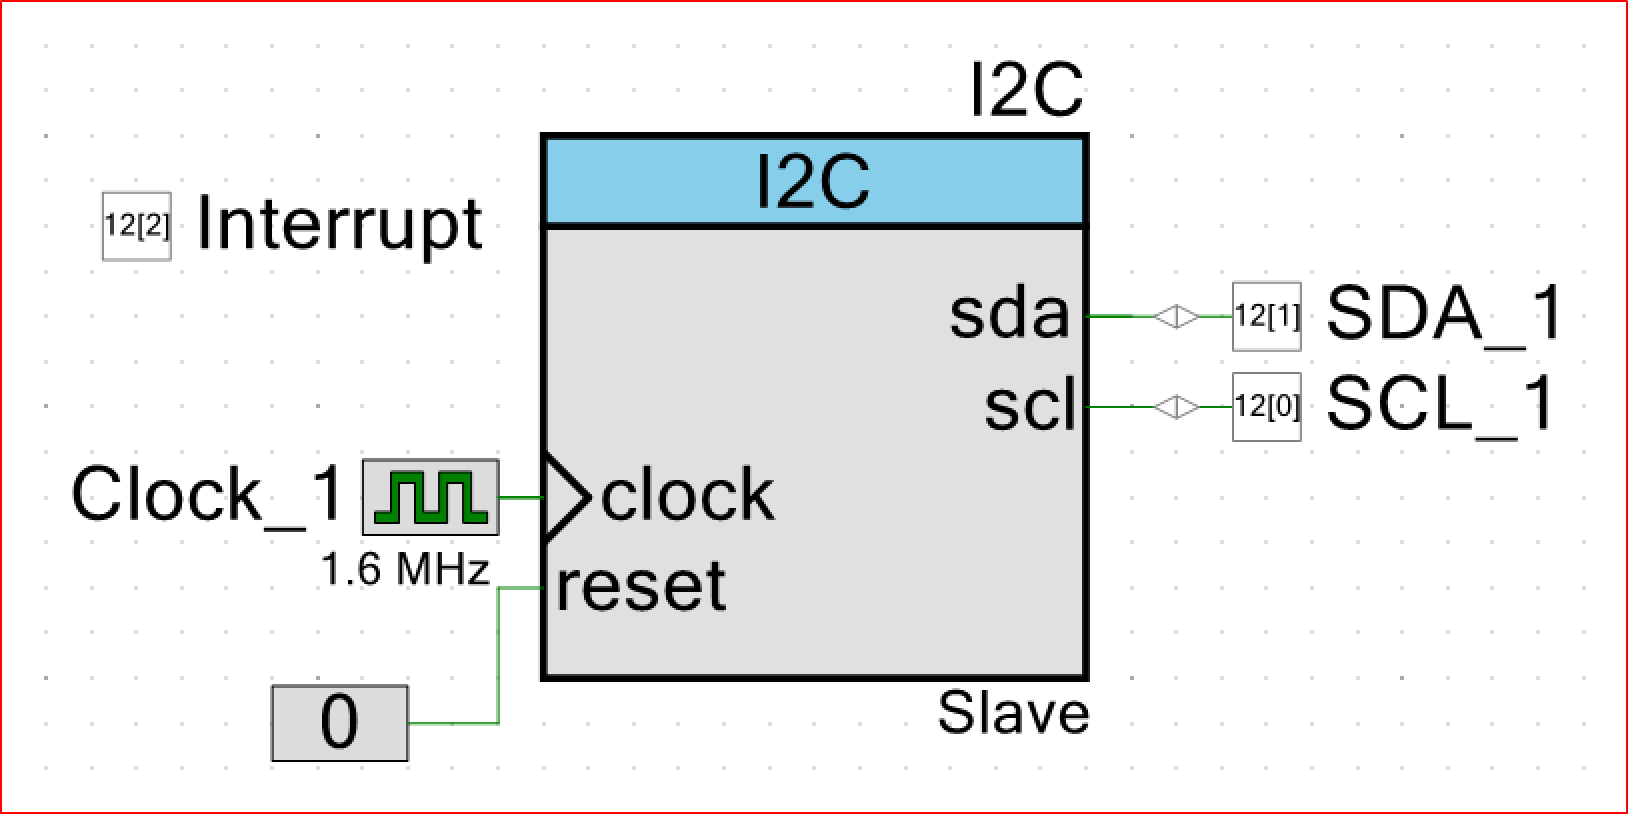
\includegraphics[width=\textwidth]{Rapport/BallDispenser/ballDispenserController/graphics/I2Cslave.png}
    \caption{I2C slave modul}
    \label{fig:I2CSlaveBallDisp}
\end{figure}
\subsubsection{Implementering}
Dette modulet består av flere funksjoner men det er noen av dem som kun er switch statements som bestemer hvilken melding som sendes, disse tas ikke med.\\
{\textbf{Definisjoner}}\\
\begin{lstlisting}[caption={Defininisjoner BallDispenser Controller},style=customc,label={lst:dispenserControlFunction}]
#define DISPENSE_OFF 0x15
#define DISPENSE_ON 0x14
#define COIN_DETECTED 0x1E
#define DISPENSER_EMPTY 0x1F
#define DISPENSER_NOT_EMPTY 0x20
\end{lstlisting}

Disse definisjonene brukes når det skal kommuniseres via I2C, demonstrasjon av dette kan sees senere i dette avsnittet.\\

{\textbf{coinInserted}}\\
\begin{lstlisting}[caption={Hoved kontrol funksjonen til ballDispenser},style=customc,label={lst:coinInserted}]
void coinInserted()
{
    handleCoinDetection();
    if(countBalls() <= 2)
        {
            disableDispenser(); 
            sendDispenserStatus();
        }
    sendCoinDetected();
    dispenseBalls();
    resetDetectionISR();
}
\end{lstlisting}
Denne funksjonen er hoved funksjonen i kontrolleren, den blir kalt når det skjer et interrupt fra detectorISR. Den går da gjennom sekvensen av funkjoner som kreves for å handtere en detektering, inkludert å kommunisere med RPi.\\

{\textbf{SendToRPi}}\\
\begin{lstlisting}[caption={Komunikasjon fra Ball Dispenser til RPi},style=customc,label={lst:sendtorpi}]
void SendToRPi(uint8_t message)
{
    resetReadBuffer();
    readBuffer[0] = message;
    I2C_SlaveClearReadBuf();
    CyDelay(1);
    Interrupt_Write(0);
    CyDelay(15);
    Interrupt_Write(1);
}
\end{lstlisting}

Denne funksjonen står for å sende beskedene til RPi, den mottar en variabel message som er den beskjeden den sender. I denne funksjonen brukes I2C slave modulet.\\

{\textbf{handleI2CData}}\\
\begin{lstlisting}[caption={Komunikasjon fra RPi til Ball Dispenser},style=customc,label={lst:handleI2CData}]
void handleI2CData()
{
    if(I2C_SlaveClearWriteStatus() & I2C_SSTAT_WR_CMPLT)
    {
        
        int writeSize = I2C_SlaveGetWriteBufSize();
        for(int i = 0; i < writeSize; i++)
        {
            switch (writeBuffer[i])
            {
                case DISPENSE_ON:{
                    UART_PutString("Enable\r\n");
                    enableDispenser();
                    break;}
                case DISPENSE_OFF:{
                    UART_PutString("Disable\r\n");
                    disableDispenser();
                    break;} 
            }
        }
    }
}
\end{lstlisting}
Denne funksjonen blir kaldt i main og looper konstant, den skjekker om det er en endring i writebufferen som er koblet til I2C slaven, hvis det har skjedd en ending så leser den innholdet og kalder funksjonene om enabler eller disabler dispenseren. Her kan det sees definisjonene fra begynnelsen av avsnittet er brukt.

\end{document}